\chapter{Siphon}
\section{Purpose}

To demonstrate that TELEMAC-2D can solve the flow in a culvert considered as
an internal singularity, under the form of a couple of source and sink nodes.
Also to show that TELEMAC-2D computes tracer dispersion.

\section{Approach}

Two square tanks are connected hydraulically by a culvert. The culvert is
represented by a couple of source / sink nodes, one in each tank. The water
level and the tracer concentration are initially higher in the left tank.

\section{Geometry and mesh}

\begin{itemize}
\item  Two identical square tanks are located 100 metres apart.
\item  The dimension of each square tank is 200~m x 200~m
\item  The water depth at rest is 4~m in the left tank, and 2 m in the right tank
\end{itemize}

The mesh is regular. It is made up with squares split into 2 triangles.

\begin{itemize}
\item  1600 triangular elements
\item  882 nodes
\item  Maximum size range: $\sqrt{200} = 14.14$ metres
\end{itemize}

\section{Boundaries}

\begin{itemize}
\item  Solid walls with slip condition in the domain.
\end{itemize}

Bottom:

\begin{itemize}
\item Strickler formula with friction coefficient = 20
\end{itemize}

\section{Physical Parmeters}

Turbulence: Model of constant viscosity with velocity diffusivity = 1 m${}^{2}$/s

\section{Numercial Parameters}

Type of advection:
\begin{itemize}
\item  characteristics on velocities (scheme n$\mathrm{{}^\circ}$1)
\item  conservative + modified SUPG on depth (mandatory)
\item  centred semi-implicit scheme + SUPG decentring on tracer (scheme n$\mathrm{{}^\circ}$2)
\end{itemize}

Type of element:
\begin{itemize}
\item  quasi-bubble triangle for velocities
\item  Linear triangle P1 for h
\end{itemize}

\begin{itemize}
\item  GMRES solver
\item  Accuracy = 10-8
\end{itemize}

Tracer:

\begin{itemize}
\item  initial concentrations : 100\% in the left square, and 50\% in the right square
\item  co-ordinates of source / sink nodes : left = (100;100) and right = (400;100)
\item  no water discharge of sources
\item  GMRES solver
\end{itemize}

Time data:

\begin{itemize}
\item  Time step = 2.5 sec.
\item  Simulation duration = 600 sec.
\end{itemize}

Mesh and initial state are shown on Figure \ref{fig:siphon:mesh}.

\section{ Results}

The water flows from the left tank to the right tank through the culvert. The
water level decreases regularly in the left tank and increases regularly in the
right tank (Figure \ref{fig:siphon:evol}). Simultaneously, a spot of tracer with concentration
100 arrives in the right tank and disperses.

In the left tank, the culvert is vertical. Therefore, the flow is regular and
symmetric around the sink node. In the right tank, the culvert is horizontal in
the direction of y-axis. Therefore, the flow takes this direction from the
source node and the velocity field forms two eddies around the source (Figure
\ref{fig:siphon:evol_vel}).

Water mass and tracer mass are conserved: no water mass is lost whereas the
cumulated loss of tracer mass at the end of the simulation is below 0.9~\% of
the initial mass.

\section{ Conclusions}

TELEMAC-2D can be used for the treatment of an internal singularity, such as a
culvert, and also for the treatment of dispersion by currents and diffusion of
a tracer.

\section{ Figures}

\begin{figure}
\centering
 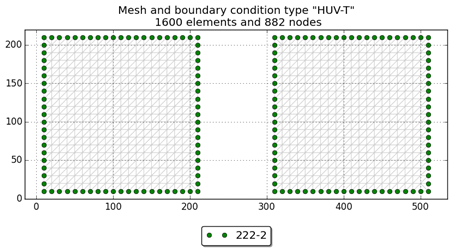
\includegraphics{img/image88}
 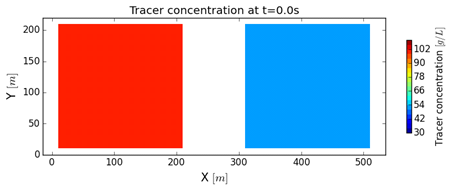
\includegraphics{img/image89}
 \caption{Mesh and initial state.}\label{fig:siphon:mesh}
\end{figure}


\begin{figure}
\centering
 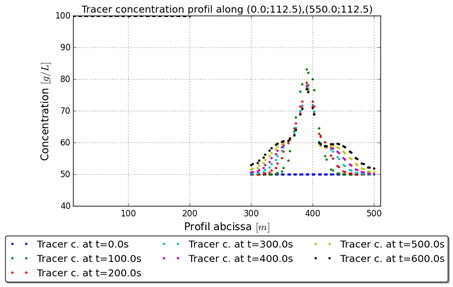
\includegraphics{img/image90}
 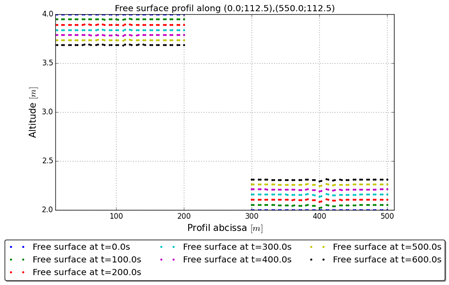
\includegraphics{img/image91}
 \caption{Evolution of the tracer concentration, and evolution of the free surface elevation in time in both tanks.}\label{fig:siphon:evol}
\end{figure}

\begin{figure}
\centering
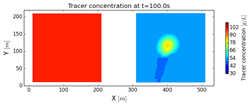
\includegraphics{img/image92}
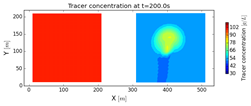
\includegraphics{img/image93}
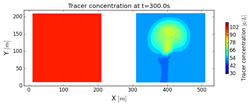
\includegraphics{img/image94}
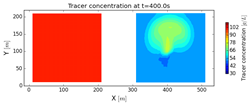
\includegraphics{img/image95}
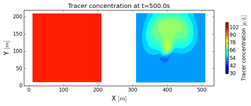
\includegraphics{img/image96}
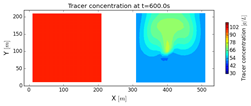
\includegraphics{img/image97}
 \caption{Evolution of the tracer concentration, and evolution of the free surface elevation in time in both tanks.}\label{fig:siphon:evolbis}
\end{figure}

\begin{figure}
\centering
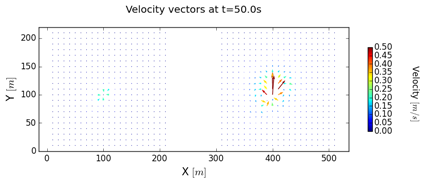
\includegraphics{img/image98}
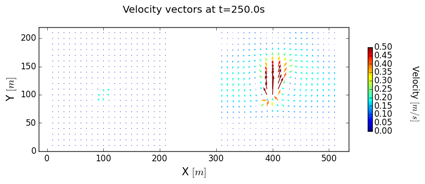
\includegraphics{img/image99}
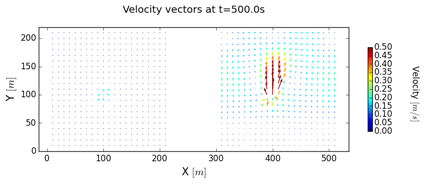
\includegraphics{img/image100}
 \caption{Evolution of velocity field in time in both tanks.}\label{fig:siphon:evol_vel}
\end{figure}
